\chapter{GIVE Challenge}
\label{chap:give-challenge}
Important framework for this thesis is the GIVE Challenge \citep{koller2010first}. The data I used to study the referencing strategies were collected using the GIVE framework \citep{koller2010first}. I used GIVE framework to implement and test a hypothesis regarding these strategies. Therefore, in this chapter I will describe this academic competition in detail.  

The first section will answers basic questions such as what is the GIVE Challenge, why was it created and what are its interesting properties. 

In the next section, I will provide a brief history of the GIVE Challenge together with some of its results. 

In the third section, the focus will be a detailed description of the shared task and the virtual world of the GIVE Challenge.

\section{Introduction}
The GIVE Challenge was a series of Natural Language Generation (NLG) competitions run from November 2008 to March 2012. Participants developed NLG systems to navigate human-controlled avatars in a 3D virtual environment. The real-time navigation was realized through written instructions displayed on the screen. Goal of the navigation was to finish a treasure-hunt game. In Figure \ref{fig:give-client} we can see the GIVE client with virtual world and example of an instruction. A more detailed description of the task and the environment is in the Section \ref{sec:task-give-world}.

\begin{figure}[!htbp]
  \centering
	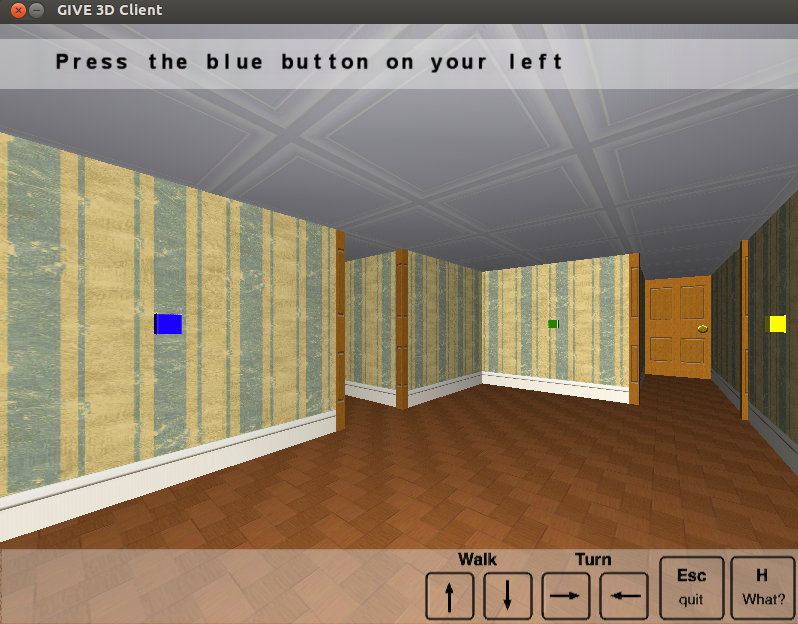
\includegraphics[width=0.7\textwidth]{Images/give-client}
	\caption{A human subject is being navigated through the environment.}
	\label{fig:give-client}
\end{figure}

\citet{koller2010first} state that one of the goals of the GIVE Challenge was spawning an interest in NLG, a subfield of computational linguistics (CL), and was inspired by other competitions in the field such as the Recognizing Textual Entailment challenge\footnote{\url{http://pascallin.ecs.soton.ac.uk/Challenges/}} and NIST machine
translation competition\footnote{\url{http://www.itl.nist.gov/iad/mig//tests/mt/}}.

According to \citet{koller2010first}, another important goal was to introduce and explore a new way of evaluating NLG algorithms, techniques and systems in a shared task. More specifically a shared task which was, on the one hand, complex enough to encompass multiple NLG subtasks and, on the other hand, was only concerned with NLG and not any other fields of computational linguistic.

Three basic approaches to evaluation of NLG systems are compared annotated corpora, measuring task performance in an experiment and human judges evaluation. \citet{koller2010first} argue the advantages and disadvantages of these evaluation in more depth, therefore I will only provide a brief summary. The first approach compares output of the NLG system to an annotated corpora, also known as a gold-standard. It is fast and cheap approach, but a problem with it lies in the complexity of the natural language. We can often express concepts in many different ways and there is often no telling which way is a better one. The second approach conducts an experiment and measures task performance on human subjects. Measuring task performance avoids the problems of gold-standard, but it is expensive and time consuming. Lastly, trained human judges are used to evaluate the system. It is less demanding than the second approach, but for the cost of certainty, that the results correspond with results one might achieve with non-expert subjects.

The GIVE Challenge proposes and successfully implements a new approach, in a sense that it wasn't used for NLG before, through Internet-based evaluation. The basic premise is using a client-server software methodology. The client is a program installed on test subject computer, which is easily downloadable from a public website. The client connects through the Internet to a matchmaker server and random evaluation world is selected. Matchmaker also connects the client to a randomly selected NLG system, which itself, can be hosted on a different server. Client and NLG systems then communicate back and forth until the task is finished. Matchmaker finally logs the entire sessions to database. Figure \ref{fig:give-clientserver} shows that architecture in a simple diagram.

\begin{figure}[!htbp]
  \centering
	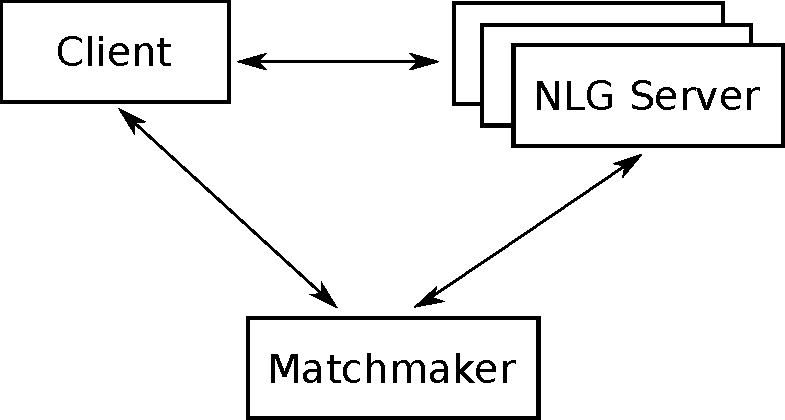
\includegraphics[width=0.7\textwidth]{Images/give-client-servers}
	\caption{Software architecture of GIVE Challenge.}
	\label{fig:give-clientserver}
\end{figure}

This approach immediately presents several advantages. It does not require physical presence of the test subject in a laboratory. The subject simply downloads the client from a website and is able to do the experiment at his/her convenience. Second obvious advantage is a scalability. The number of individuals which can parallelly undertake the experiment is only limited by the servers' load. Thanks to the low costs, advertisement becomes the decisive limitation on the number of subjects. Take for example the second instalment of the GIVE Challenge which had up to 1800 participants.

On the other hand, part of the control over the experiment is lost in this approach; for example the control over subject pool. Another problem which rises with this approach is that individuals can repeat the experiment.

In addition to Internet-based evaluation, the GIVE Challenge utilized variety of evaluation measures of both objective and subjective nature. Among objective measure were task success rate, number of instructions or time required to finish the task. For subjective measures a questionnaire was used at the end of the session. The questionnaire mostly used a 5 point scale with question such as how clear where the instruction or how friendly was the system. Some of the measures intentionally collided with each other, putting emphasize on a certain characteristic of the system.

Having presented the basic concept of the GIVE Challenge and reasons for its creation, I will now move onto a brief history of this competition. 

 
\section{History of GIVE Challenge}
The first instalment of GIVE Challenge (GIVE-1) was publicized in March 2008. \citet{koller2010first} report on this instalment and are the source of following information. For more details please refer to their paper. The data collection period was from November 2008 to February 2009. Four teams participated in this challenge, namely from these universities: University of Texas at Austin, Universidad Complutense de Madrid, University of Twente and Union College. The team from University of Twente submitted two systems, making the final number of systems five.

What is important to note about GIVE-1 is a different world representation from the following instalments. GIVE-1 used discrete square grid for player movement. Player was able to rotate only by $90^{\circ}$ and walk forward and backwards by one square of the grid. That had a major impact on the design of NLG systems. Participating teams at least occasionally used this grid in their references (eg. \textit{move forward three steps}). Afterwards organizers realized that the grid and the discrete movement made the task easier than intended and they were after GIVE-1 removed.

Altogether, 1143 valid games were recorded. The demographics featured a majority of males (over 80\%) and wide spread over different countries in the world. For the actual results,  the system from Austin significantly outperformed all other systems in task completion time. At the same time systems from Union and Madrid outperformed other systems in success rate. That shows the significance of different measures for the evaluation. Similar interesting conclusion in both objective and subjective measures can be found in previously mentioned paper. Apart from objective and subjective measures, the report examined influence of English language proficiency and differences between evaluation worlds. The English proficiency had an impact on the task success rate but solely for the least proficient category. The evaluation world also had a significant influence on the task success rate.

Finally, the first instalment also compared the Internet-based evaluation with more standard laboratory evaluation. The conclusion was that Internet-based evaluation provides meaningful results comparable and even more precise in some areas to the laboratory setting.

The second instalment (GIVE-2) run from August 2009 (data collection starting in February 2010) to May 2010 and is thoroughly described by \citet{koller2010report}. Following information are based on this paper. Biggest difference to the GIVE-1, which was mentioned previously, is that players were now able to move freely. This made the instruction generation considerably harder. Additionally, the questionnaire was revised and a few new objectives measures were introduced. Evaluation worlds used in GIVE-2 were considerably harder than in GIVE-1. Number of distracting buttons was increased and same-colored buttons were in some cases next to each other. Also number of alarm tiles was increased. Otherwise, the architecture and the rest of the details stayed the same as in GIVE-1.

This time 1825 games were played over seven NLG systems developed by six teams from: Dublin Institute of Technology, Trinity College Dublin, Universidad Complutense de Madrid, University of Heidelberg, Saarland University and INRIA Grand-Est in Nancy (2 systems).

There was a big drop in success rate, most likely linked to the free movement and the increase of difficulty in the evaluation worlds. Similarly to results in GIVE-1, there was an influence of English proficiency and game world on the task success rate. Additionally, age of the subject played a role in the time required to finish the task and number of actions to finish the task (younger subjects being faster and requiring less actions). The difference between genders in time required to finish was not present in GIVE-2.

Some teams participating in the GIVE Challenge tried to use a corpora of a human to human interactions in GIVE scenario. They were learning language expression or decision-making process and applying them in their NLG systems. The teams were however relying on small self-collected datasets. In a light of this, organizers of GIVE Challenge decided they would collect and provide dataset for future use. \citet{gargett2010give} describe this dataset, which was used in the next instalment of the GIVE challenge.

Following GIVE-2 was so called Second Second instalment (GIVE-2.5), which kept almost the same settings as GIVE-2. There was just a small addition to objective measures and a reduction in the number of subjective questions. The data collection took place between July 2011 and March 2012. \citet{striegnitz2011report} report on the partial results of 536 valid games from July and August 2011, which however constitute a majority of the final number of 650 valid games.

Eight NLG systems participated from 7 teams: University of Aberdeen, University of Bremen, Universidad Nacional de Córdoba, Universidad Nacional de Córdoba and LORIA/CNRS, LORIA/CNRS, University of Potsdam (2 systems) and University of Twente. In this instalment the teams employed more broad spectrum of approaches. Team from University of Bremen used decision trees learned from GIVE-2 corpus. Universidad Nacional de Córdoba and LORIA/CNRS, LORIA/CNRS selected instructions from a corpus of human to human interactions. The teams also often included algorithms from existing NLG and CL literature.

Apart from comparing the systems through objective and subjective measures, \citet{striegnitz2011report} again examined effects of evaluation worlds and demographics factors on task success rate. The evaluation worlds and the English proficiency had an effect. Additionally computer expertise and familiarity with computer games significantly influenced the task performance. The difference between male and female subject wasn't significant.

The following section describes the shared task in more detail and lists possible objects of the GIVE virtual worlds.

\section{Task and GIVE world}
\label{sec:task-give-world}
The GIVE world is a 3D virtual world. The world is an indoor environment, comprising of rooms connected by doors. It's defined in a human-readable format and stored in a text file. The following objects can be places in a world:

\begin{itemize}
\item
Alarm tile
\item
Button
\item
Door
\item 
Landmark
	\begin{itemize}
	\item
	Bed	
	\item
	Chair	
	\item
	Couch	
	\item
	Dresser
	\item
	Flower	
	\item
	Lamp
	\item
	Table
	\item
	Window
	\end{itemize}
\item
Picture
\item
Safe
\item
Trophy
\item
Wall
\end{itemize}

In addition, some of these objects can have attributes, states or can operate other objects. Buttons have colors as an example of attribute. Doors and safes can be in a closed or an open state. Buttons can operate doors, safes or pictures.

Walls are actually created automatically by defining shapes of rooms. Rooms can have rectangular shape or can be defined by a polygon. I will sometimes use a term ``corridor'' which is a connecting room, usually not containing any button.

The landmarks serve as a decoration but they can be used in an expression generation. Picture is technically a landmark as well, but in GIVE Challenge it often serves another purpose. It covers the safe and needs to be put aside by a button press.

\begin{figure}[!htbp]
  \centering
	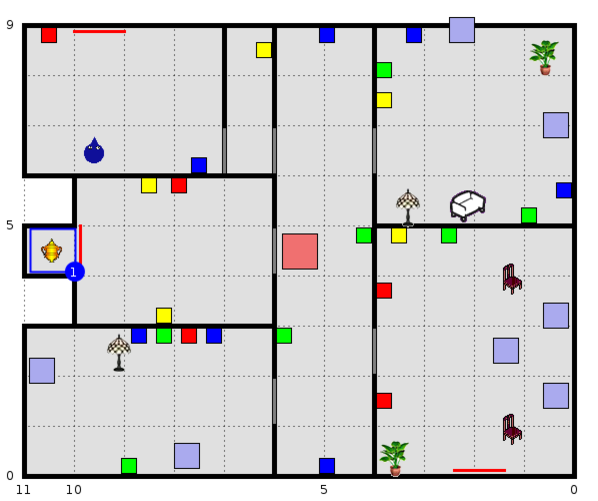
\includegraphics[width=0.75\textwidth]{Images/give-evalworldexmaple}
	\caption{Example GIVE world viewed in GIVE map viewer utility.}
	\label{fig:give-evalworldexmaple}
\end{figure}

Figure \ref{fig:give-evalworldexmaple} shows an evaluation world number one from GIVE-2.5. In top-left room we can see player starting position. Buttons are colored squares on the walls. Grey bars on the walls are closed doors. Trophy in a safe is in the middle-left room. There are also landmarks (like lamp or chair) and one big read square marking an alarm tile.

The flexibility of GIVE world creation allows relatively broad range of scenarios for the task. On the other hand, all the GIVE Challenge instalments consisted of similar sequence of steps.

The goal of all the GIVE Challenge worlds is to pick up a trophy. The trophy is hidden in a closed safe. In order to open the safe a sequence of buttons, usually counting somewhere around 6 buttons, has to be pressed. The safe can be also hidden by a picture, which needs to be put aside. The buttons in a safe-opening series are often in different rooms. Rooms can be also closed off, requiring another button press to open the door. While moving around the world, player has to avoid alarm tiles. Stepping on an activated alarm tile causes an immediate loss. Alarm tiles can block the only path and need to deactivated by a button press. Some buttons also cause an alarm and an immediate loss.

Depending on the number of rooms, complexity of buttons arrangement and length of safe-opening sequence, the task can range from short and trivial problem easily handled by a few instruction templates, to a long and hard case, where it's impossible to capture every possible scenario.

To summarize, navigation system of a player in the GIVE world has to deal with following steps. Note that their order depends on the world definition and they can be thought of as layers of behaviours the system must enforce on player.

\begin{itemize}
\item
Avoid alarm tiles
\item
Avoid pressing alarm-causing buttons
\item
Deactivate path-blocking alarm tiles by a button press
\item
Open closed-off rooms by pressing correct buttons
\item
Press a sequence of buttons to open the safe
\item
Reveal safe behind a picture by pressing correct button
\item
Take the trophy
\end{itemize}

After the safe was opened and possibly revealed from behind the picture player can pick up the trophy and therefore win the game.